% -*- latex -*-
%%%%%%%%%%%%%%%%%%%%%%%%%%%%%%%%%%%%%%%%%%%%%%%%%%%%%%%%%%%%%%%%
%%%%%%%%%%%%%%%%%%%%%%%%%%%%%%%%%%%%%%%%%%%%%%%%%%%%%%%%%%%%%%%%
%%%%
%%%% This text file is part of the source of 
%%%% `Introduction to High-Performance Scientific Computing'
%%%% by Victor Eijkhout, copyright 2012
%%%%
%%%% This book is distributed under a Creative Commons Attribution 3.0
%%%% Unported (CC BY 3.0) license and made possible by funding from
%%%% The Saylor Foundation \url{http://www.saylor.org}.
%%%%
%%%%
%%%%%%%%%%%%%%%%%%%%%%%%%%%%%%%%%%%%%%%%%%%%%%%%%%%%%%%%%%%%%%%%
%%%%%%%%%%%%%%%%%%%%%%%%%%%%%%%%%%%%%%%%%%%%%%%%%%%%%%%%%%%%%%%%

In section~\ref{sec:2dbvp} you saw that the discretization of
\ac{BVP}s (and \ac{IBVP}s) may give rise to sparse matrices.
Since such a matrix has $N^2$ elements but only $O(N)$
nonzeros, it would be a big waste of space to store this as a two-dimensional
array. Additionally, we want to avoid operating on zero elements.

In this section we will explore efficient storage schemes for sparse
matrices, and the form that familiar linear algebra operations take
when using sparse storage.

\Level 1 {Storage of sparse matrices}
\label{sec:spmvp}

\index{matrix!storage, sparse|(}

It is pointless to look for an exact definition of
\indextermbus{sparse}{matrix}, but an operational definition is that a
matrix is called `sparse' if there are enough zeros to make
specialized storage feasible. We will discuss here briefly the most
popular storage schemes for sparse matrices.
Since a matrix is no longer stored as a simple 2-dimensional array,
algorithms using such storage schemes need to be rewritten too. 

\Level 2 {Diagonal storage}
\label{sec:diagonal-storage}
\index{diagonal storage|(}
\index{banded matrix!storage|(}

In section~\ref{sec:1dbvp} you have seen examples of sparse matrices
that were banded. In fact, their nonzero elements are located
precisely on a number of subdiagonals. For such a matrix, a
specialized storage scheme is possible.

Let us take as an example the matrix of the one-dimensional \ac{BVP}
(section~\ref{sec:1dbvp}). Its elements are located on three
subdiagonals: the main diagonal and the first super and
subdiagonal. The idea of \indexterm{storage by diagonals} or
\emph{diagonal storage} is to store the diagonals consecutively
in memory. The most economical storage scheme for such a matrix would
store the $2n-2$ elements consecutively. However, for various reasons
it is more convenient to waste a few storage locations, as shown in
figure~\ref{fig:sparsediag}.

\begin{figure}[ht]
  \begin{quote}
    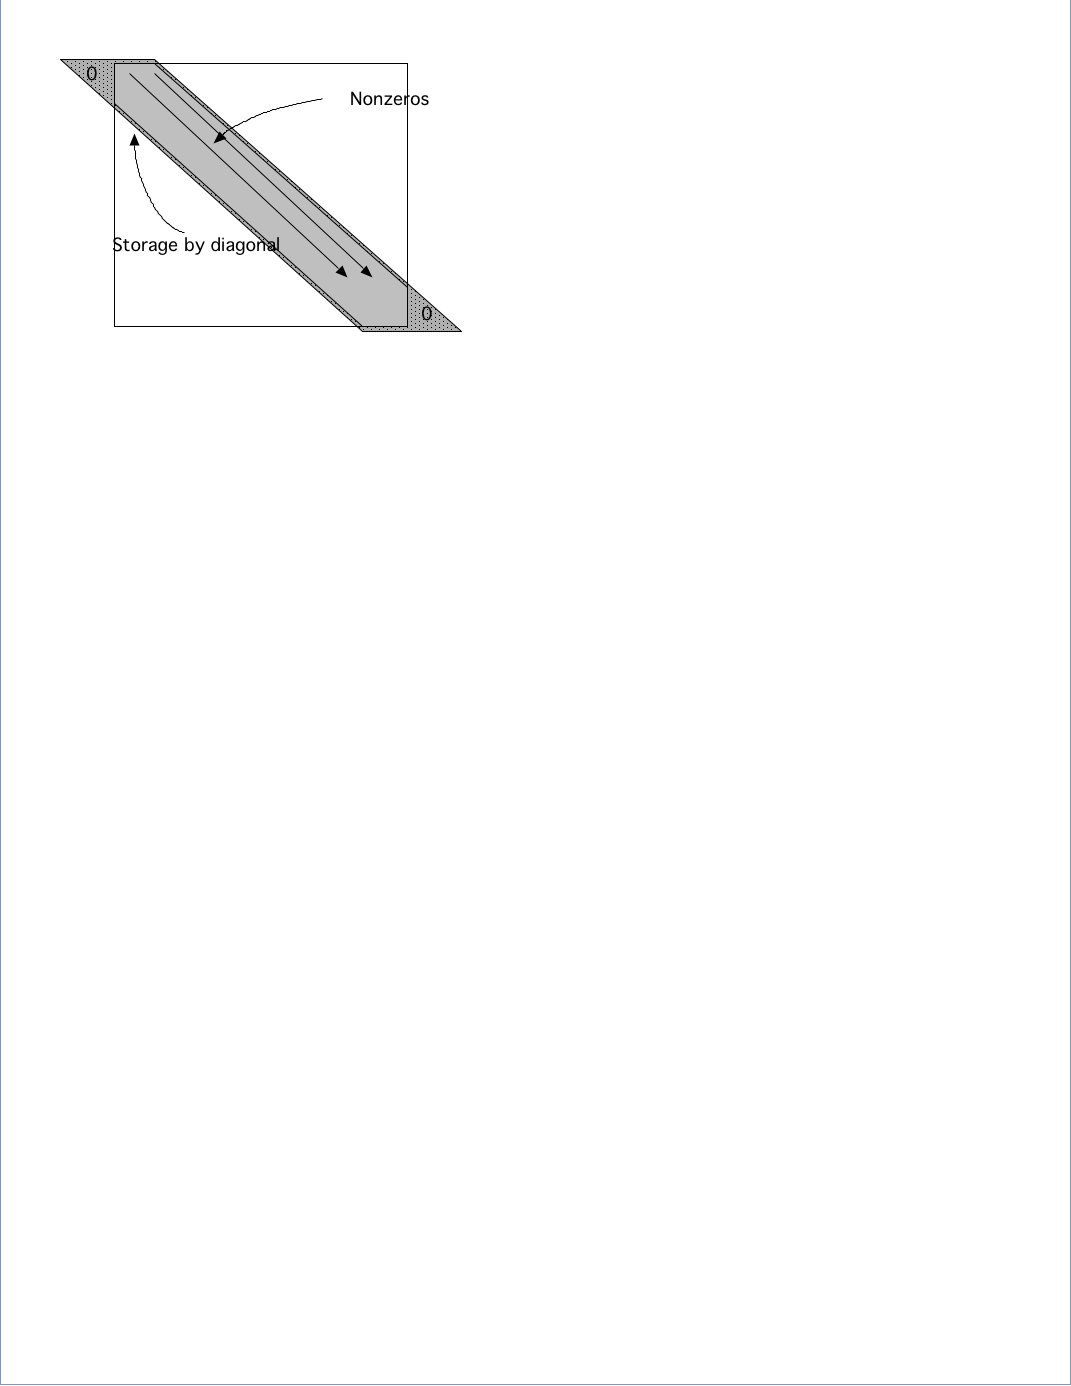
\includegraphics[scale=.1]{graphics/sparsediag}
  \end{quote}
  \caption{Diagonal storage of a banded matrix}
  \label{fig:sparsediag}
\end{figure}

Thus, for a matrix with size $n\times n$ and a
\emph{bandwidth}\index{bandwidth!of a matrix}~$p$\index{bandwidth!of a
  matrix|see{halfbandwidth}}, we need a
rectangular array of size $n\times p$ to store the matrix. The matrix
of equation~\eqref{eq:1d2nd-matrix-vector} would then be stored as
\begin{equation}
\begin{array}{|ccc|}
  \hline
  \star&2&-1\\
  -1&2&-1\\
  \vdots&\vdots&\vdots\\
  -1&2&\star\\ \hline
\end{array}
\label{eq:2minus1-by-diagonals}
\end{equation}
where the stars indicate array elements that do not correspond to
matrix elements: they are the triangles in the top left and bottom
right in figure~\ref{fig:sparsediag}. 

Of course, now we have to wonder about the conversion between array
elements \n{A(i,j)} and matrix elements~$A_{ij}$. This is easiest done
in the Fortran language. If we allocate the array with
\begin{verbatim}
dimension A(n,-1:1)
\end{verbatim}
then the main diagonal $A_{ii}$ is stored in \n{A(*,0)}. For instance,
%
$\n{A(1,0)}\sim A_{11}$. The next location in the same row of the matrix~$A$, 
%
$\n{A(1,1)}\sim A_{12}$. It is easy to see that together we have the
conversion
\begin{equation}
  \n{A(i,j)}\sim A_{i,i+j}.
  \label{eq:sparse-conversion}
\end{equation}

\begin{exercise}
  What is the reverse conversion, that is, what array location
  \n{A(?,?)} does the matrix element~$A_{ij}$ correspond to?
\end{exercise}

\begin{exercise}
  If you are a C~programmer, derive the conversion between matrix
  elements $A_{ij}$ and array elements~\n{A[i][j]}.
\end{exercise}

If we apply this scheme to the matrix of the two-dimensional \ac{BVP}
(section~\ref{sec:2dbvp}), it becomes wasteful, since we would be
storing many zeros that exist inside the band. Therefore, we refine
this scheme by storing only the nonzero diagonals: if the matrix has
$p$ nonzero diagonals, we need an $n\times p$ array. For the matrix of
equation~\eqref{eq:5starmatrix} this means:
\[
\begin{array}{|ccccc|}
  \hline
  \star&\star&4&-1&-1\\
  \vdots&\vdots&4&-1&-1\\
  \vdots&-1&4&-1&-1\\
  -1&-1&4&-1&-1\\
  \vdots&\vdots&\vdots&\vdots&\vdots\\
  -1&-1&4&\star&\star\\ \hline
\end{array}
\]
Of course, we need an additional integer array telling us the
locations of these nonzero diagonals.

In the preceding examples, the matrices had an equal number of nonzero
diagonals above and below the main diagonal. In general this need not
be true. For this we introduce the concepts of
\begin{itemize}
\item \indextermsub{left}{halfbandwidth}: if $A$ has a left
  halfbandwidth of $p$ then $A_{ij}=0$ for $i>j+p$, and
\item \indextermsub{right}{halfbandwidth}: if $A$ has a right
  halfbandwidth of~$p$ then $A_{ij}=0$ for~\mbox{$j>i+p$}.
\end{itemize}

\index{banded matrix!storage|)}
\index{diagonal storage|)}

\Level 2 {Operations on diagonal storage}

The most important operation on sparse matrices is the matrix-vector
product. With a matrix stored by diagonals, as described above, it is
still possible to perform the ordinary rowwise or columnwise product using the
conversion formula~\eqref{eq:sparse-conversion}\footnote{In fact,
  this is how Lapack banded routines work.}.
%
However, with
a small bandwidth, this gives short vector lengths and relatively high
loop overhead, so it will not be efficient. It is possible do to much
better than that.

If we look at how the matrix elements are used in the matrix-vector
product, we see that the main diagonal is used as
\[ y_i \leftarrow y_i + A_{ii} x_i, \]
the first superdiagonal is used as
\[ y_i \leftarrow y_i + A_{ii+1} x_{i+1}\quad\hbox{for $i<n$}, \]
and the first subdiagonal as
\[ y_i \leftarrow y_i + A_{ii-1} x_{i-1}\quad\hbox{for $i>1$}. \]
In other words, the whole matrix-vector product can be executed in
just three vector operations of length~$n$ (or $n-1$), instead of $n$
inner products of length 3 (or~2).

\begin{verbatim}
for diag = -diag_left, diag_right
    for loc = max(1,1-diag), min(n,n-diag)
        y(loc) = y(loc) + val(loc,diag) * x(loc+diag)
    end
end
\end{verbatim}

\begin{exercise}
  Write a routine that computes $y\leftarrow A^tx$ by
  diagonals. Implement it in your favourite language and test it on a
  random matrix.
\end{exercise}
\begin{exercise}
  The above code fragment is efficient if the matrix is dense inside
  the band. This is not the case for, for instance, the matrix of 
  two-dimensional \acp{BVP}; see section~\ref{sec:2dbvp} and in
  particular equation~\eqref{eq:5starmatrix}. Write code for the
  matrix-vector product by diagonals that only
  uses the nonzero diagonals.
\end{exercise}
\begin{exercise}
  Multiplying matrices is harder than multiplying a matrix times a
  vector. If matrix $A$ has left and halfbandwidth $p_A,q_Q$, and
  matrix $B$ has $p_B,q_B$, what are the left and right halfbandwidth
  of $C=AB$? Assuming that an array of sufficient size has been
  allocated for~$C$, write a routine that computes $C\leftarrow AB$.
\end{exercise}

\index{diagonal storage|)}

\Level 2 {Compressed row storage}
\label{sec:crs}
\indexacstart{CRS}

If we have a sparse matrix that does not have a simple band structure,
or where the number of nonzero diagonals becomes impractically large,
we use the more general \acf{CRS} scheme. As the name indicates, this
scheme is based on compressing all rows, eliminating the zeros; see
figure~\ref{fig:crs}.
\begin{figure}[ht]
  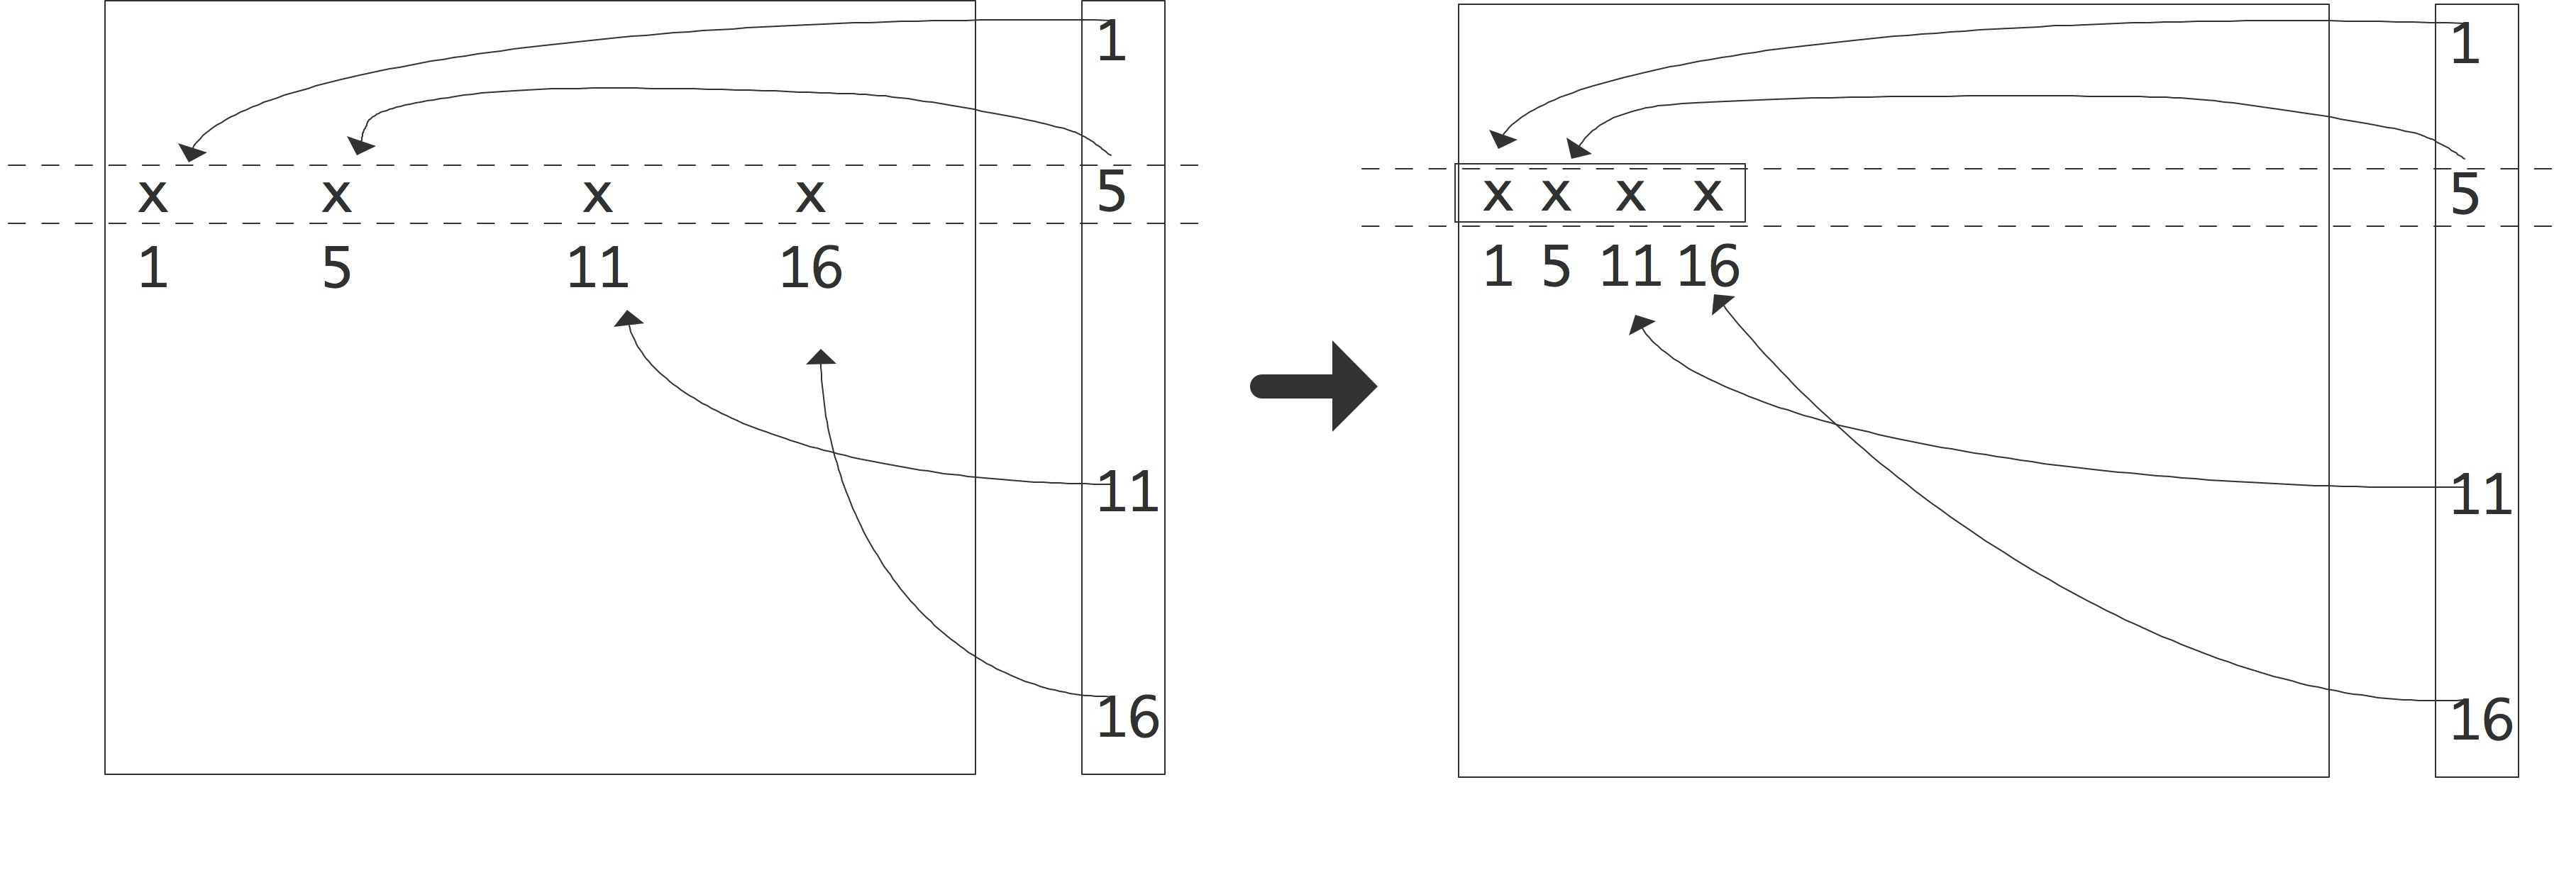
\includegraphics[scale=.13]{graphics/crs}
  \caption{Compressing a row of a sparse matrix in the CRS format}
  \label{fig:crs}
\end{figure}
Since this loses the information what columns the nonzeros originally
came from, we have to store this explicitly.
Consider an example of a sparse matrix:
\begin{equation}
A =
\left(\begin{array}{rrrrrr}
      10 &  0 &  0 & 0  &-2 &  0 \\
       3 &  9 &  0 & 0  & 0 &  3 \\
       0 &  7 &  8 & 7  & 0 &  0 \\
       3 &  0 &  8 & 7  & 5 &  0 \\
       0 &  8 &  0 & 9  & 9 & 13 \\
       0 &  4 &  0 & 0  & 2 & -1
           \end{array}
\right) ~.
\end{equation}
After compressing all rows, we store all
nonzeros in a single real array. The column indices are
similarly stored in an integer array, and we store pointers to where
the columns start. Using 0-based indexing this gives:
\begin{center}
\begin{tabular}{|r|r|r|r|r|r|r|r|r|r|r|r|r|r|r|r|} \hline
{\tt val}     &10 &-2& 3& 9& 3& 7& 8& 7& 3 $\cdots$  9&13& 4& 2&-1 \\ \hline
{\tt col\_ind}& 0 & 4& 0& 1& 5& 1& 2& 3& 0 $\cdots$  4& 5& 1& 4& 5 \\ \hline
\end{tabular} \\
\vspace{.02 in}
\begin{tabular}{|r|r|r|r|r|r|r|r|} \hline
{\tt row\_ptr}& 0 & 2 & 5 & 8 & 12 & 16 & 19  \\ \hline
\end{tabular} ~.
\end{center}
A simple variant of \ac{CRS} is \indexac{CCS} where the elements in columns
are stored contiguously. This is also known as the
\indexterm{Harwell-Boeing matrix format}~\cite{Duff:harwellboeingformat}.
Another storage scheme you may come across is
\indexterm{coordinate storage}, where the matrix is stored as a list
of triplets $\langle i,j,a_{ij}\rangle$.The popular \indexterm{Matrix
Market}\index{Matrix Market!matrix format}
website~\cite{matrix-market} uses a variant of this scheme.

\Level 2 {Algorithms on compressed row storage}
\label{sec:crs-mvp}

In this section we will look at the form
some algorithms take in \ac{CRS}.

First we consider the \emph{implementation of the sparse matrix-vector
  product}.\index{sparse!matrix-vector product!implementation}
\begin{verbatim}
for (row=0; row<nrows; row++) {
   s = 0;
   for (icol=ptr[row]; icol<ptr[row+1]; icol++) {
      int col = ind[icol];
      s += a[icol] * x[col];
   }
   y[row] = s;
}
\end{verbatim}
You recognize the standard matrix-vector product algorithm for $y=Ax$,
where the inner product is taken of each row~$A_{i*}$ and the input
vector~$x$. However, note that the inner loop no long has the column
number as index, but rather the location where that number is to be
found. This extra step is known as \indexterm{indirect addressing}.

\begin{exercise}
  Compare the data locality of the dense matrix-vector product, executed by rows,
  with the sparse product given just now. Show that, for general sparse matrices,
  the spatial locality in addressing\index{sparse!matrix-vector product!locality in}
  the input vector~$x$ has now disappeared. Are there matrix structures for which
  you can still expect some spatial locality?
\end{exercise}

Now, how about if you wanted to compute the product $y=A^tx$? In that
case you need rows of~$A^t$, or, equivalently, columns of~$A$. Finding
arbitrary columns of $A$ is hard, requiring lots of searching, so you may
think that this algorithm is correspondingly hard to
compute. Fortunately, that is not true.

If we exchange the $i$ and $j$ loop in the standard algorithm for
$y=Ax$, we get
\[
  \vcenter{
    \begin{tabbing}
      $y\leftarrow 0$\\
      for \=$i$:\\
      \> for \=$j$:\\
      \>\> $y_i\leftarrow y_i+a_{ij}x_j$
    \end{tabbing}
  }\qquad\Rightarrow\qquad
  \vcenter{
    \begin{tabbing}
      $y\leftarrow 0$\\
      for \=$j$:\\
      \> for \=$i$:\\
      \>\> $y_i\leftarrow y_i+a_{ji}x_j$
    \end{tabbing}
  }
\]
We see that in the second variant, columns of $A$ are accessed, rather
than rows. This means that we can use the second algorithm for
computing the~$A^tx$ product by rows.

\begin{exercise}
  Write out the code for the transpose product $y=A^tx$ where $A$~is
  stored in \ac{CRS} format. Write a simple test program and confirm
  that your code computes the right thing.
\end{exercise}

\begin{exercise}
  What if you need access to both rows and columns at the same time?
  Implement an algorithm that tests whether a matrix stored in CRS
  format is symmetric. Hint: keep an array of pointers, one for each
  row, that keeps track of how far you have progressed in that row.
\end{exercise}

\begin{exercise}
The operations described so far are fairly simple, in that they never
make changes to the sparsity structure of the matrix. The CRS format,
as described above, does not allow you to add new nonzeros to the
matrix, but it is not hard to make an extension that does allow it.

Let numbers $p_i, i=1\ldots n$, describing the number of nonzeros in
the $i$-th row, be given.  Design an extension to CRS that gives each
row space for $q$ extra elements. Implement this scheme and test it:
construct a matrix with $p_i$ nonzeros in the $i$-th row, and check
the correctness of the matrix-vector product before and after adding
new elements, up to $q$ elements per row.

Now assume that the matrix will never have more than a total of $qn$
nonzeros. Alter your code so that it can deal with starting with an
empty matrix, and gradually adding nonzeros in random places. Again,
check the correctness.
\end{exercise}

We will revisit the transpose product algorithm in
section~\ref{sec:shared-crs-transpose} in the context of shared memory
parallelism.

\indexacend{CRS}

\index{matrix!storage, sparse|)}

\Level 1 {Sparse matrices and graph theory}
\label{sec:sparse-graph}
\index{graph theory!of sparse matrices}

Many arguments regarding sparse matrices can be formulated in terms of
graph theory.  To see why this can be done,
consider a matrix~$A$ of size~$n$ and observe that we can
define a graph $\langle E,V\rangle$ by $V=\{1,\ldots,n\}$, $E=\{(i,j)\colon
a_{ij}\not=0\}$. This is called the \indexterm{adjacency graph} of the
matrix. For simplicity, we assume that $A$ has a nonzero
diagonal. 
If
necessary, we can attach weights to this graph, defined by
$w_{ij}=a_{ij}$. The graph is then denoted $\langle E,V,W\rangle$.
(If you are not familiar with the basics of graph
theory, see appendix~\ref{app:graph}.)

Graph properties now correspond to matrix properties; for instance,
the degree of the graph is the maximum number of nonzeros per row, not
counting the diagonal element. As another example, if the graph of the
matrix is an \indextermsub{undirected}{graph}, this means that
$a_{ij}\not=0\Leftrightarrow a_{ji}\not=0$. We call such a matrix
\emph{structurally symmetric}\index{matrix!structurally symmetric|textbf}:
it is not truly symmetric in the
sense that $\forall_{ij}\colon a_{ij}=a_{ij}$, but every nonzero in
the upper triangle corresponds to one in the lower triangle and vice versa.

One advantage of considering the graph of a matrix is that graph properties
do not depend on how we order the nodes, that is, they are invariant
under permutation of the matrix.

\begin{exercise}
  Let us take a look at what happens with a matrix~$A$ when the nodes
  of its graph $G=\langle V,E,W\rangle$ are renumbered. As a simple example,
  we number the nodes backwards; that is, with $n$ the number of
  nodes, we map node~$i$ to $n+1-i$.
  Correspondingly, we find a new graph
  $G'=\langle V,E',W'\rangle$ where
  \[ (i,j)\in E'\Leftrightarrow (n+1-i,n+1-j)\in E,\qquad
  w'_{ij}=w_{n+1-i,n+1-j}.\]
  What does this renumbering imply for the matrix~$A'$ that
  corresponds to~$G'$? If you exchange the labels $i,j$ on two nodes,
  what is the effect on the matrix~$A$?
\end{exercise}

Some graph properties can be hard to see from the sparsity pattern of
a matrix, but are easier deduced from the graph.

\begin{exercise}
  \label{ex:rb-tridiagonal}
  Let $A$ be the tridiagonal matrix of the one-dimensional \ac{BVP}
  (see section~\ref{sec:1dbvp}) of size~$n$ with $n$~odd. What does
  the graph of~$A$ look like?  Consider the permutation that results
  from putting the nodes in the following sequence:
  $1,3,5,\ldots,n,2,4,\allowbreak6,\ldots,\allowbreak n-\nobreak
  1$. What does the sparsity pattern of the permuted matrix look like?
  Renumbering strategies such as this will be discussed in more detail
  in section~\ref{sec:redblackgreen}.
\end{exercise}

\begin{exercise}
  \label{ex:reducible-tridiagonal}
  Take again the matrix from the previous exercise, and zero the
  offdiagonal elements closest to the `middle' of the matrix: let
  $a_{(n+1)/2,(n+1)/2+1}=a_{(n+1)/2+1,(n+1)/2}=0$. Describe what that
  does to the graph of~$A$. Such a graph is called
  \indexterm{reducible}. Now apply the permutation of the previous
  exercise and sketch the resulting sparsity pattern. Note that the
  reducibility of the graph is now harder to read from the sparsity
  pattern.
\end{exercise}

\Level 1 {LU factorizations of sparse matrices}
\label{sec:fill}

In section~\ref{sec:1dbvp} the one-dimensional \ac{BVP} led to a
linear system with a tridiagonal coefficient matrix. If we do one
step of Gaussian elimination, the only element that needs to be
eliminated is in the second row:
\[
\begin{pmatrix}
  2&-1&0&\ldots\\ -1&2&-1\\ 0&-1&2&-1\\ 
  &\ddots&\ddots&\ddots&\ddots
\end{pmatrix}
\quad\Rightarrow\quad
\left(\begin{array}{c|cccc}
  2&-1&0&\ldots\\ \hline 0&2-\frac12&-1\\ 0&-1&2&-1\\ 
  &\ddots&\ddots&\ddots&\ddots
\end{array}\right)
\]
There are two important observations to be
made: one is that this elimination step does not change any zero
elements to nonzero. The other observation is that the part of the
matrix that is left to be eliminated is again
tridiagonal. Inductively, during the elimination no zero elements
change to nonzero: the sparsity pattern of $L+U$ is the same as
of~$A$, and so the factorization takes the same amount of space to
store as the matrix.

\begin{comment}
this one already appears elsewhere
\begin{exercise}
  Since, in the factorization of a tridiagonal matrix, $L+U$ has the
  same storage demands as~$A$, we intuitively double the storage, if
  we do not overwrite~$A$. However, it is possible to be even more
  parsimonious. Recall equation~\eqref{eq:A=LUnormalized} where $A$
  was factored as $A=(I+L)D(I+U)$. Show that, in this case of a
  tridiagonal matrix, $L$~and $U$ contain unaltered elements of~$A$:
  $\ell_{ij}=a_{ij}$ for $i>j$ and $u_{ij}=a_{ij}$ for~$j>i$. What
  does this imply for the required storage?
\end{exercise}
\end{comment}

The case of tridiagonal matrices is unfortunately not typical, as we
will shortly see in the case of two-dimensional problems. But first we
will extend the discussion on graph theory of
section~\ref{sec:sparse-graph} to factorizations.

\Level 2 {Graph theory of sparse LU factorization}
\label{sec:lu-graph}
\index{LU factorization!graph interpretation}

Graph theory is often useful when discussion the
%
\emph{LU factorization of a sparse matrix}.
%
Let us investigate what eliminating the first unknown
(or sweeping the first column) means in graph theoretic terms. We are
assuming a structurally symmetric matrix.

We consider eliminating an unknown as a process
that takes a graph $G=\langle V,E\rangle$ and
turns it into a graph $G'=\langle V',E'\rangle$. The relation between
these graphs is first that a vertex, say~$k$,
has been removed from the vertices:
$k\not\in V'$, $V'\cup \{k\}=V$.

The relationship between $E$ and $E'$ is more complicated. In the
Gaussian elimination algorithm the result of eliminating variable~$k$ is
that the statement
\[ a_{ij} \leftarrow a_{ij}- a_{ik}a_{kk}\inv a_{kj} \]
is executed for all $i,j\not=k$. If $a_{ij}\not=0$ originally, then
its value is merely altered. In case $a_{ij}=0$ in the original
matrix, there will be a nonzero element, termed a \indexterm{fill-in}
element, after the $k$ unknown
\begin{figure}[ht]
  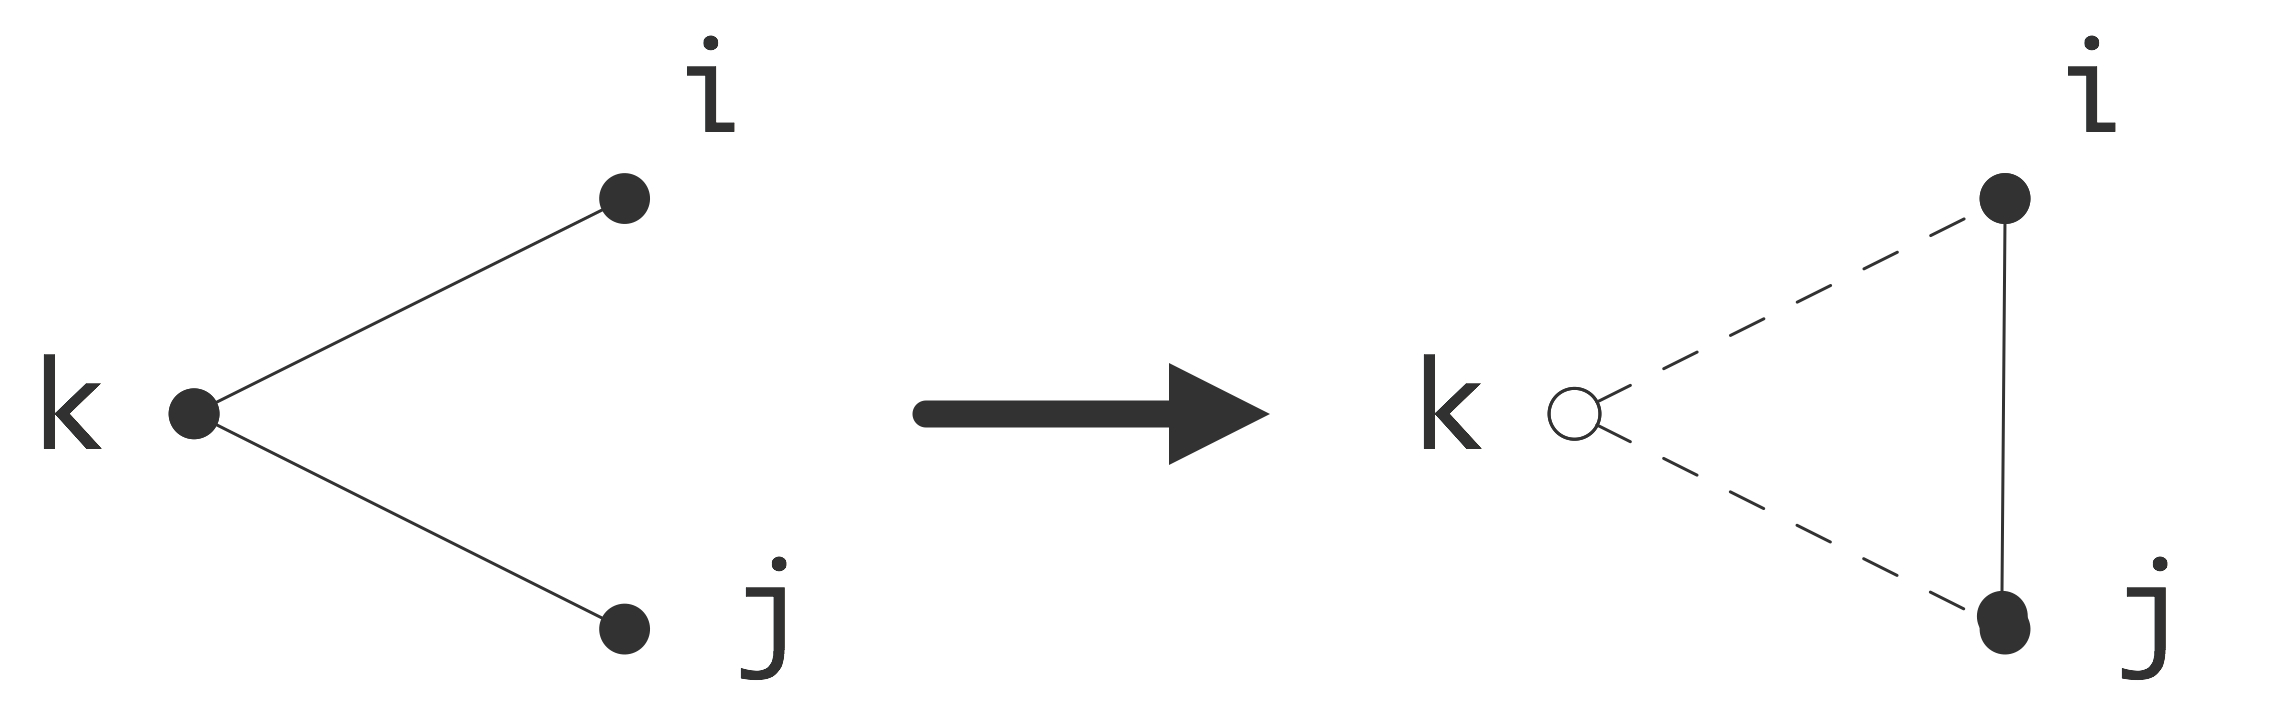
\includegraphics[scale=.12]{graphics/ijk-eliminate}
  \caption{Eliminating a vertex introduces a new edge in the quotient
    graph}
  \label{fig:ijk-eliminate}
\end{figure}
is eliminated: in $E$ there was no edge $(i,j)$, and
this edge \emph{is} present in~$E'$. This is illustrated in
figure~\ref{fig:ijk-eliminate}.

Summarizing, eliminating an unknown gives a graph that has one vertex
less, and that has edges for all $i,j$ such that there were edges
between $i$ or $j$ and the eliminated variable~$k$.

\begin{exercise}
  Go back to exercise~\ref{ex:rb-tridiagonal}. Use a graph argument to
  determine the sparsity pattern after the odd variables have been
  eliminated.
\end{exercise}

\begin{exercise}
  \label{ex:schur-fill}
  Prove the generalization of the above argument about eliminating a
  single vertex. Let $I\subset V$ be any set of
  vertices, and let $J$ be the vertices connected to~$I$:
  \[ J\cap I=\emptyset,\quad \forall_{i\in I}\exists_{j\in J}\colon (i,j)\in
  E. \]
  Now show that eliminating the variables in~$I$ leads to a graph
  $\langle V',E'\rangle$ where all nodes in~$J$ are connected in the
  remaining graph, if there was a path between them through~$I$:
  \[ \forall_{j_1,j_2\in J}\colon \hbox{there is a path
    $j_i\rightarrow j_2$ through $I$ in $E$} \Rightarrow 
    (j_1,j_2)\in E'.
  \]
\end{exercise}

\Level 2 {Fill-in}
\index{fill-in|(}

We now return to the factorization of the matrix from two-dimensional
problems. We write such
matrices of size $N\times N$ as block matrices with block
dimension~$n$, each block being of size~$n$.
%
(Refresher question:
where do these blocks come from?)
%
Now, in the first
elimination step we need to zero two elements, $a_{21}$ and~$a_{n+1,1}$.

{\small
\[
\left(\begin{array}{ccccc:cccc}
  4&-1&0&\ldots&&-1\\ -1&4&-1&0&\ldots&0&-1\\ 
  &\ddots&\ddots&\ddots&&&\ddots\\ \hdashline
  -1&0&\ldots&&&4&-1\\ 0&-1&0&\ldots&&-1&4&-1\\
\end{array}\right)
\quad\Rightarrow\quad
\left(\begin{array}{c|cccc:cccc}
  4&-1&0&\ldots&&-1\\ \hline &4-\frac14&-1&0&\ldots&-1/4&-1\\ 
  &\ddots&\ddots&\ddots&&&\ddots&\ddots\\ \hdashline
  &-1/4&&&&4-\frac14&-1\\ &-1&0&&&-1&4&-1\\
\end{array}\right)
\]
}

You see that eliminating $a_{21}$ and $a_{n+1,1}$ causes two
\emph{fill} elements to appear: in the original matrix $a_{2,n+1}$ and
$a_{n+1,2}$ are zero, but in the modified matrix these locations
are nonzero.  We define \indexterm{fill locations} as
locations $(i,j)$ where $a_{ij}=0$, but~$(L+U)_{ij}\not=0$.

Clearly the matrix fills in during factorization. With a
little imagination you can also see that every element in the band
outside the first diagonal block will fill in. However, using the
graph approach of section~\ref{sec:lu-graph} it becomes easy to
visualize the fill-in connections that are created.

In figure~\ref{fig:row-eliminate} this is illustrated for the 
graph of the 2d \ac{BVP} example. (The edges corresponding to diagonal
elements have not been pictured here.)
\begin{figure}
  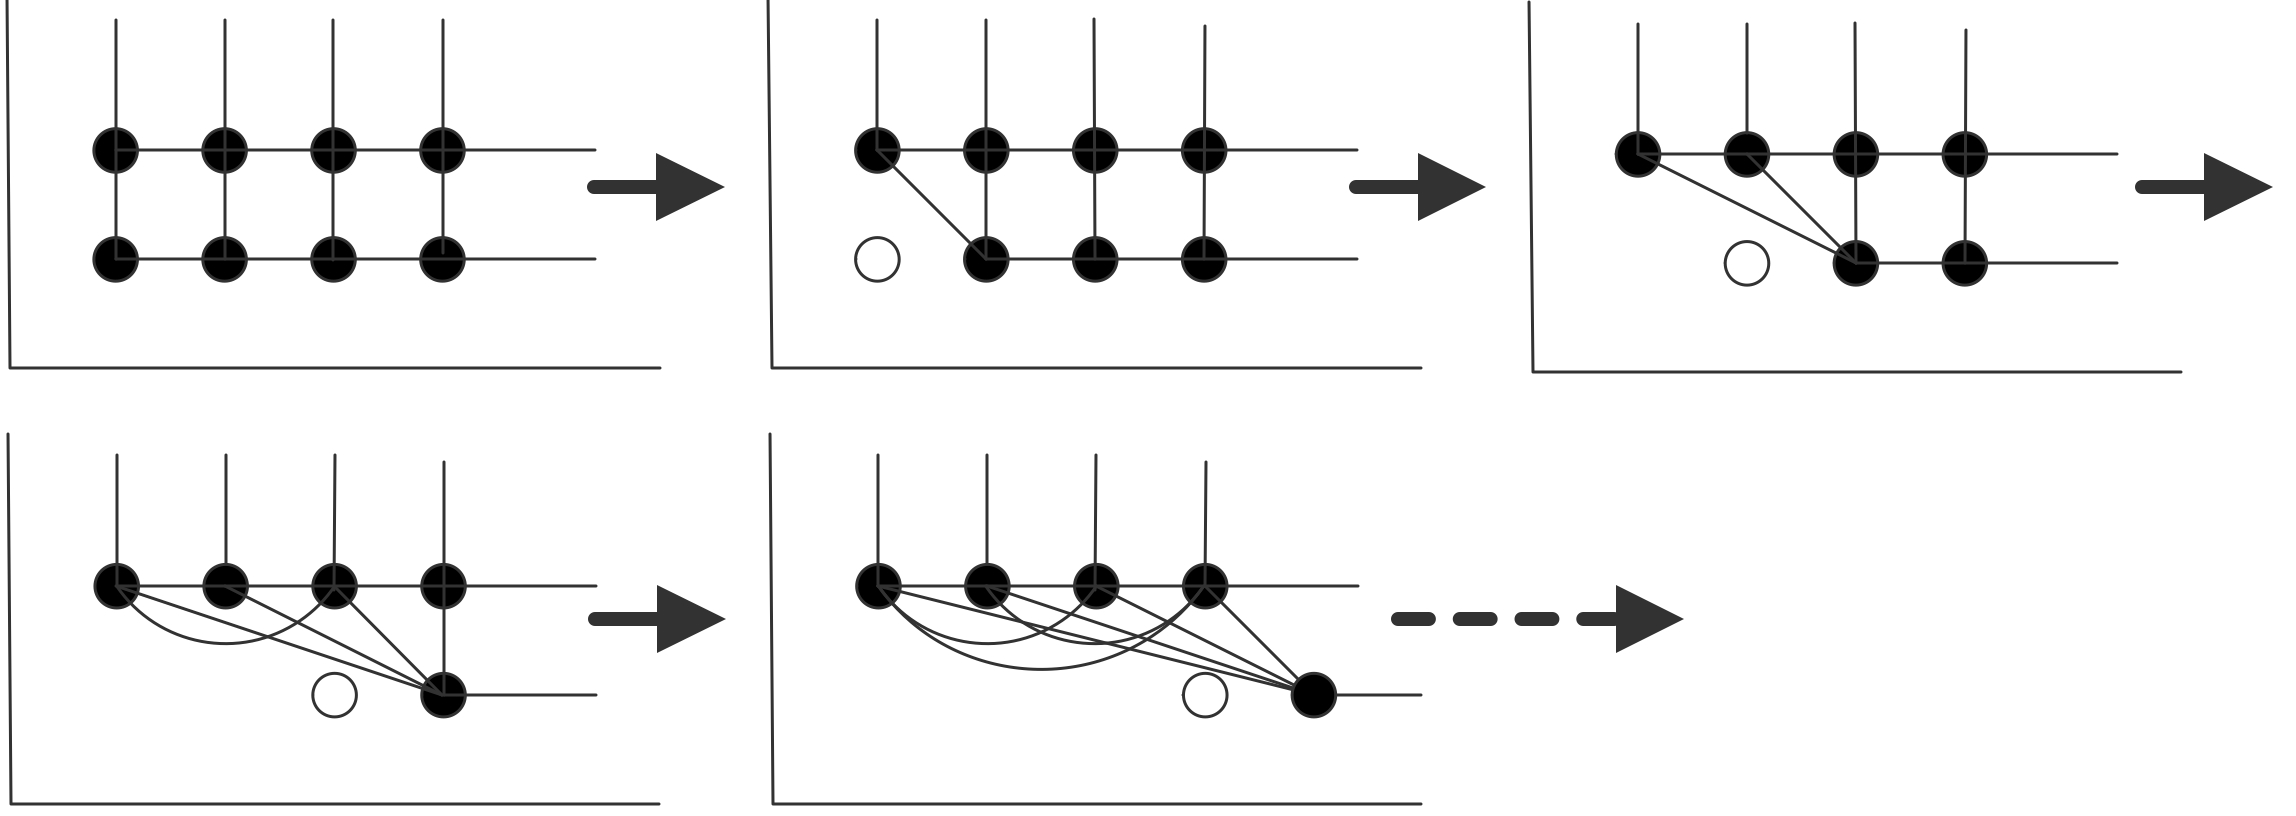
\includegraphics[scale=.2]{graphics/row-eliminate}
  \caption{Creation of fill-in connection in the matrix graph}
  \label{fig:row-eliminate}
\end{figure}
Each variable in the first row that is eliminated creates connections
between the next variable and the second row, and between variables in
the second row. Inductively you see that after the first row is
eliminated the second row is fully connected. (Connect this to
exercise~\ref{ex:schur-fill}.)

\begin{exercise}
  Finish the argument. What does the fact that variables in the second
  row are fully connected imply for the matrix structure? Sketch in a
  figure what happens after the first variable in the second row is
  eliminated.
\end{exercise}

\begin{exercise}
  The LAPACK software for dense linear algebra has an LU factorization
  routine that overwrites the input matrix with the factors. Above you
  saw that is possible since the columns of~$L$ are generated
  precisely as the columns of~$A$ are eliminated. Why is such an
  algorithm not possible if the matrix is stored in sparse format?
\end{exercise}

\Level 2 {Fill-in estimates}
\label{sec:bandfill}
\index{complexity!space|(}
\index{fill-in!estimates|(}

In the above example you saw that the factorization of a sparse matrix
can take much more space than the matrix itself, but still less than
storing an entire square array of size the matrix dimension. We will now give
some bounds for the \indextermsub{space}{complexity} of the
factorization, that is, the amount of space needed to execute the
factorization algorithm.

\begin{exercise}
\label{ex:skyline}
  Prove the following statements.
  \begin{enumerate}
  \item Assume that the matrix $A$ has a
    \indexterm{halfbandwidth}~$p$, that is, $a_{ij}=0$ if
    $|i-j|>p$. Show that, after a factorization without pivoting,
    $L+U$ has the same halfbandwidth.
  \item Show that, after a factorization with partial pivoting,
    $L$~has a left halfbandwidth of~$p$, whereas $U$~has a
    right halfbandwidth of~$2p$.
  \item Assuming no pivoting, show that the fill-in can be
    characterized as follows:
    \begin{quote}
      Consider row~$i$. Let $j_{\min}$ be the leftmost nonzero in
      row~$i$, that is $a_{ij}=0$ for $j<j_{\min}$. Then there will be
      no fill-in in row~$i$ to the left of
      column~$j_{\min}$. Likewise, if $i_{\min}$ is the topmost
      nonzero in column~$j$, there will be no fill-in in column~$j$
      above row~$i_{\min}$.
    \end{quote}
    As a result, $L$~and~$U$ have a `skyline' profile. Given a sparse
    matrix, it is now easy to allocate enough storage to fit a
    factorization without pivoting: this is knows as
    \indexterm{skyline storage}.
  \end{enumerate}
\end{exercise}

This exercise shows that we can allocate enough storage for the
factorization of a banded matrix:
\begin{itemize}
\item for the factorization without pivoting of a matrix with
  bandwidth~$p$, an array of size $N\times p$ suffices;
\item the factorization with partial pivoting of a matrix left
  halfbandwidth~$p$ and right halfbandwidth~$q$ can be stored in
  $N\times (p+2q+1)$.
\item A skyline profile, sufficient for storing the factorization, can
  be constructed based on the specific matrix.
\end{itemize}

We can apply this estimate to the matrix from the two-dimensional
\ac{BVP}, section~\ref{sec:2dbvp}.  
\begin{exercise}\label{ex:bandfill}
  Show that in equation~\eqref{eq:5starmatrix} the original matrix has
  $O(N)=O(n^2)$ nonzero elements, $O(N^2)=O(n^4)$~elements in total,
  and the factorization has $O(nN)=O(n^3)=O(N^{3/2})$ nonzeros.
\end{exercise}

These estimates show that the storage required for an $LU$
factorization can be more than what is required for~$A$, and the
difference is not a constant factor, but related to the matrix
size. Without proof we state that the inverses of the kind of sparse
matrices you have seen so far are fully dense, so storing them takes
even more. This is an important reason that solving linear systems
$Ax=y$ is not done in practice by computing $A\inv$ and multiplying
$x=A\inv y$. (Numerical stability is another reason that this is not
done.) The fact that even a factorization can take a lot of
space is one reason for considering iterative methods, as we will do
in section~\ref{sec:iterative}.

Above, you saw that the factorization of a dense matrix of size
$n\times n$ takes $O(n^3)$ operations. How is this for a sparse
matrix? Let us consider the case of a matrix with halfbandwidth~$p$,
and assume that the original matrix is dense in that band.
The pivot element $a_{11}$ is used to zero $p$ elements in the first
column, and for each the first row is added to that row, involving $p$
multiplications and additions. In sum, we find that the number of
operations is roughly
\[ \sum_{i=1}^n p^2 = p^2\cdot n \]
plus or minus lower order terms.

\begin{exercise}
  The assumption of a band that is initially dense is not true for the
  matrix of a two-dimensional \ac{BVP}. Why does the above estimate
  still hold, up to some lower order terms?
\end{exercise}

In exercise~\ref{ex:skyline} above you derived an estimate for the
amount of fill-in that is easy to apply. However, it can be a
considerable overestimate. It is desirable to compute or estimate the
amount of fill-in with less work than doing the actual factorization.
We will now sketch an algorithm for finding the exact
number of nonzeros in $L+U$, with a cost that is linear in this
number. We will do this in the (structurally) symmetric case. The
crucial observation is the following. Suppose column~$i$ has more than
one nonzero below the diagonal:
\[
\begin{pmatrix}
  \ddots\\ &a_{ii}&&a_{ij}&&a_{ik}\\ 
  &&\ddots\\ &a_{ji}&&a_{jj}\\ &&&&\ddots\\
  &a_{ki}&&?a_{kj}?&&a_{kk}\\ 
\end{pmatrix}
\]
Eliminating $a_{ki}$ in the $i$-th step causes an update of~$a_{kj}$,
or a fill-in element if originally $a_{kj}=0$. However, we can infer
the existence of this nonzero value: eliminating $a_{ji}$ causes a
fill-in element in location~$(j,k)$, and we know that structural
symmetry is preserved. In other words, if we are only
counting nonzeros, it is enough to look at the effects of elimating
the $(j,i)$ location, or in general the first nonzero below the
pivot. Following this argument through, we only need to record the
nonzeros in one row per pivot, and the entire process has a complexity
linear in the number of nonzeros in the factorization.

\index{complexity!space|)}
\index{fill-in!estimates|)}

\Level 2 {Fill-in reduction}
\label{sec:arrow-matrix}
\index{fill-in!reduction|(}

Graph properties of a matrix, such as degree and diameter, are
invariant under renumbering the variables. Other properties, such as
fill-in during a factorization, are affected by renumbering.
In fact, it is worthwhile investigating whether it is possible
to reduce the amount of fill-in by renumbering the nodes of the matrix
graph, or equivalently,
by applying a
\indexterm{permutation} to the linear system.

\begin{exercise}
  Consider the `arrow' matrix with nonzeroes only 
  in the first row and column and on the diagonal:
  \[ 
  \begin{pmatrix}
    *&*&\cdots&*\\ *&*&&\emptyset\\ \vdots&&\ddots\\ *&\emptyset&&*
  \end{pmatrix}
  \]
  What is the number of nonzeros in the matrix, and in the
  factorization, assuming that no addition ever results in zero? Can
  you find a symmetric permutation of the variables of the problem
  such that the new matrix has no fill-in?
\end{exercise}

This example is not typical, but it is true that fill-in
estimates can sometimes be improved upon by clever permuting
of the matrix (see for instance section~\ref{sec:dissection}).
Even with this, as a rule
the statement holds that an $LU$ factorization of a sparse
matrix takes considerably more space than the matrix itself. This is
one of the motivating factors for the iterative methods in the next
section.

\Level 2 {Fill-in reducing orderings}
\label{sec:fill-ordering}

Some matrix properties are invariant under symmetric permutations.
\begin{exercise}
  In linear algebra classes, you typically look at matrix properties
  and whether they are invariant under a change of basis, in
  particular under \indexterm{unitary basis transformations}:
  \[ B = VAV^t,\quad\hbox{where $VV^t=I$.} \]
  Show that a
  symmetric permutation a particular change of basis is. Name some
  matrix properties that do not change under unitary transformations.
\end{exercise}
Other properties are not: in the previous section you saw that the
amount of fill-in is one of those. Thus, you may wonder what the best
ordering is to reduce the fill-in of factoring a given matrix. This
problem is intractable in practice, but various heuristics exist. Some
of these heuristics can also be justified from a point of view of
parallelism; in fact, the
\indexterm{nested dissection} ordering will only be discussed in the
section on parallelism~\ref{sec:dissection}.
Here we briefly show two other heuristics that predate the
need for parallelism.

\index{Cuthill-McKee ordering|(}
The \emph{Cuthill-McKee ordering}~\cite{CuMcK:reducing} orders
the variables in \indexterm{level sets}. It considers the
\indextermsub{adjacency}{graph} of the matrix, and proceeds as
follows:
\begin{enumerate}
\item Take an arbitrary node, and call that `level zero'.
\item Given a level~$n$, assign all nodes that are connecting to
  level~$n$, and that are not yet in a level, to
  level~$n+\nobreak1$.
\item For the so-called `reverse Cuthill-McKee ordering', reverse the
  numbering of the levels.
\end{enumerate}
\begin{exercise}
  Show that permuting a matrix according to the Cuthill-McKee ordering
  has a \indexterm{block tridiagonal} structure.
\end{exercise}
We will revisit this algorithm in section~\ref{sec:wavefront} when we
consider parallelism.
\index{Cuthill-McKee ordering|)}

Another ordering is motivated by the observation that the amount of
fill-in is related to the degree of nodes.
\begin{exercise}
  Show that eliminating a node with degree~$d$ leads to at most $2d$
  fill elements
\end{exercise}

The so-called \indexterm{minimum degree ordering} proceeds as follows:
\index{matrix ordering!minimum degree|see{minimum degree ordering}}
\begin{itemize}
\item Find the node with lowest degree;
\item eliminate that node and update the degree information for the
  remaining nodes;
\item repeat from the first step, with the updated matrix graph.
\end{itemize}

\begin{exercise}
  Indicate a difference between the two above-mentioned methods. Both
  are based on inspection of the matrix graph; however, the minimum
  degree method requires much more flexibility in the data structures
  used. Explain why and discuss two aspects in detail.
\end{exercise}

\index{fill-in!reduction|)}
\index{fill-in|)}
